\documentclass[11pt,ngerman,a4paper]{article}
%Gummi|061|=)
\usepackage{amsmath}
\usepackage{a4wide}
\usepackage{url}
\usepackage{amsthm}
\usepackage{amsbsy}
\usepackage{amssymb}
\usepackage[utf8]{inputenc}
\usepackage{rotating} 
\usepackage{here}
\usepackage{graphicx}
\usepackage{paralist}
\usepackage{selinput}
\usepackage[separate-uncertainty=true]{siunitx}
\usepackage{booktabs}

\sisetup{}
\SelectInputMappings{%
adieresis={ä},
germandbls={ß},
}
\title{\textbf{Versuch V604: Beugung am Spalt}}
\author{Martin Bieker\\
		Julian Surmann\\
		\\
		Durchgef\"{u}hrt am 10.06.2014\\
		TU Dortmund}
\date{}
\usepackage{graphicx}
\begin{document}
\renewcommand\tablename{Tabelle}
\renewcommand\figurename{Abbildung}
\maketitle
\thispagestyle{empty}
\newpage
\clearpage
\setcounter{page}{1}


\section{Einleitung}
Im folgenden Versuch wird die Beugung von Licht an Einzelspalten und einem Doppelspalt untersucht. Unter Beugung versteht man die Abweichung der Ausbreitung von Licht hinter kleinen Öffnungen von den Gesetzen der geometrischen Optik.
\section{Theorie}
Im Fall der Beugung muss Licht als Welle betrachtet werden. Beugungphänomene können dann z.B. mit dem Huygensschen Prinzip und dem Interferenzprinzip erklärt werden. 
\subsection{Beugung am Einzelspalt}
Es sind zwei Formen der Beugung zu unterscheiden: Die Fresnel-Beugung und die Fraunhofer-Beugung (Abbildung \ref{abb1}).\newline
Bei der Fresnel-Beugung befinden sich die Lichtquelle und der Beobachtungspunkt (Schirm) im Endlichen. Dabei interferieren im Beobachtungspunkt Strahlen, die unter verschiedenen Winkeln gebeugt wurden. Bei der Fraunhofer-Beugung liegt die Lichtquelle im Unendlichen, d.h. es werden parallele Strahlenbündel emittiert. Mathematisch ist der zweite Fall viel einfacher zu behandeln, auf die Fresnel-Beugung soll hier nicht weiter eingegangen.
Der Länge des verwendete Spaltes beträgt ein Vielfaches der Breite, sodass nur ein eindimensionales Beugungsbild entsteht.
Es fällt eine ebene Welle mit der Feldstärke
\begin{equation}
A(z,t) = A_0 e^{i(wt- \frac{2\pi z}{ \lambda} )}
\end{equation}
pro Längeneinheit der Wellenfront aus der Z-Richtung ein.
Um das Prinzip der Fraunhofer-Beugung zu verwenden, ist der Abstand Beugungsebene-Beobachtungsebene sehr viel größer als die Spaltbreite b.\newline
Um die Amplitude des in Richtung $\phi$ gebeugten Lichtes zu berechnen, muss man über alle Strahlenbündel summieren, die von allen Orten der Spaltöffnung in Richtung $\phi$ emittiert werden. Zwei beliebige Strahlenbündel, die im Spalt eine Strecke x voneinander entfernt sind, haben aufgrund der Wegdifferenz zur Beobachtungsebene eine Phasendifferenz $\delta$ mit
\begin{equation}
\delta = \frac{2 \pi s}{\lambda} = \frac{2 \pi x \sin \phi}{\lambda}
\end{equation}
Aufgrund der infinitesimal kleinen Breiten der Strahlenbündel geht in der Berechnung der Amplitude die Summe in ein Integral über:
\begin{equation}
B (z, t, \phi) = A_0 
\end{equation}
\subsection{Beugung am Doppelspalt}
\subsection{Fraunhofersche Beugung und Fourier-Transformation}
\section{Aufbau}
\section{Auswertung}
\subsection{Mikroskopische Vermessung der Spalte}
Das in diesem Versuch zur Vermessung der Beugungsobjekte verwendete Mikroskop besitzt willkürlich unterteilte Skala. Daher muss dieses zunächst mit Hilfe eines Objektmikrometers geeicht werden. Als Umrechnungsfaktor $f$ ergibt sich:
\[
f = \num{3.53e-05}\,\frac{\si{\meter}}{\mathrm{Einheit}}
\]
Die gemessenen und umgerechneten Werte für die Spaltbreite $b$ und den Abstand der Spalte beim Doppelspalt $g$ befinden sich in Tabelle 1.
\begin{table}[h]
\centering
\begin{tabular}{lSSSS}

\toprule
&$\frac{b}{\mathrm{Einheit}}$ & $\frac{b}{\si{\meter}}$ & $\frac{g}{\mathrm{Einheit}}$ &$\frac{g}{\si{\meter}}$\\
\midrule
Einzelspalt A & 1.9  &6.71e-5 & &\\
Einzelspalt B & 3.8  &1.34e-4 &&\\
Doppelspalt   & 4.6  & 1.63e-4&20.8&7.35e-4\\
\bottomrule
\end{tabular}
\caption{Ergebnisse der Mikroskopischen Untersuchung}
\end{table}


\subsection{Beugungsmuster am Einzelspalt}

Die an den Einzelspalten gemessenen Werte befinden sich in Tabelle 2. Von diesen Stromstärken muss noch der so genannte thermische Dunkelstrom 
\[
I_D = \SI{}{\nano\ampere}
\]
abgezogen werden. Um die Messwerte mit der Theorie vergleichen zu können, werden die gemessenen Strecken $x$ um die Position des 0. Maximums zentriert und in einen Winkel $\phi$ umgerechnet. Dabei gilt der Zusammenhang
\[
\varphi \approx \frac{x-x_0}{L}
\] 
Der Abstand zwischen Schirm und Beugungsebene beträgt
\[
L = \SI{}{\meter} \mathrm{.}
\]
Diese Winkel und die korrigierten Stromstärken befinden sich ebenfalls in Tabelle 2. Die Abbildungen \ref{plot0} und  \ref{plot1} zeigen den Photostrom in Abhängigkeit von $\varphi$.
\begin{figure}[h]
\centering
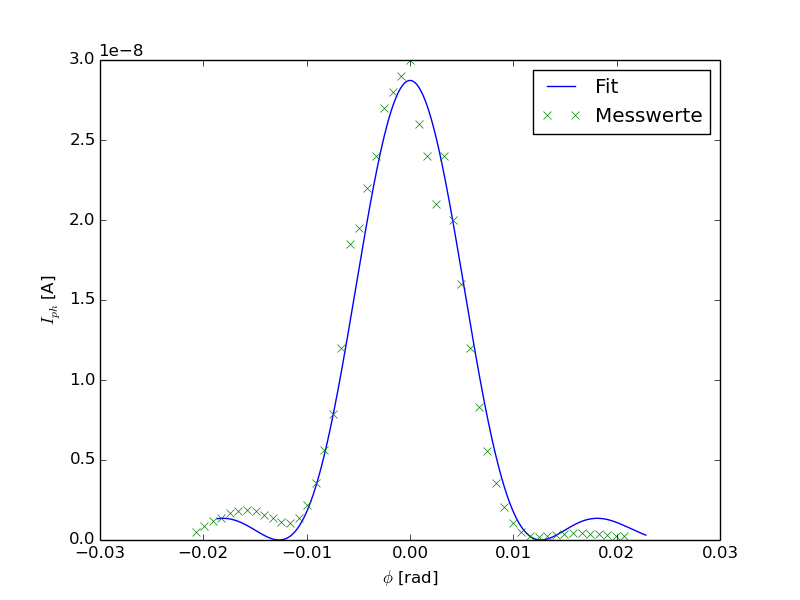
\includegraphics[scale=0.8]{plot0.png}
\caption{Beugungsmuster des Einzelspalts A ($b \approx \SI{}{\milli\meter}$)}
\label{plot0}
\end{figure}

\begin{figure}[h]
\centering
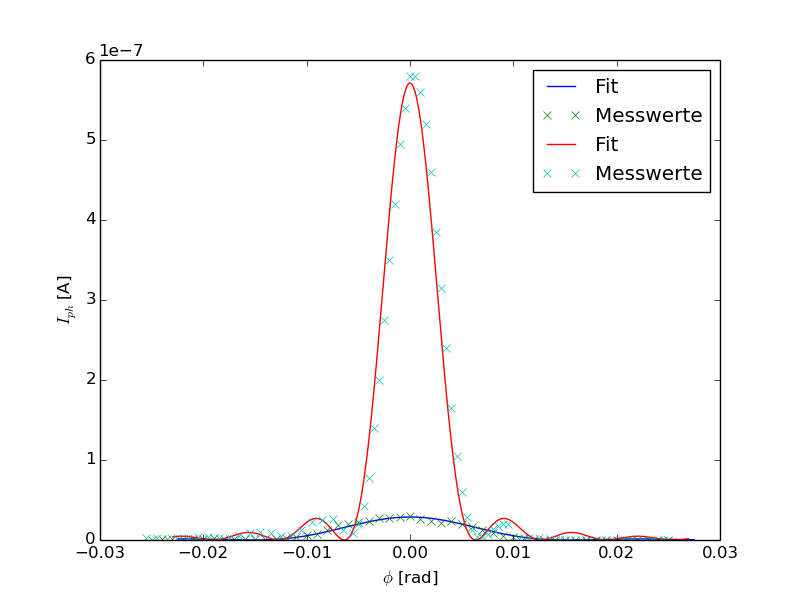
\includegraphics[scale=0.8]{plot1.png}
\caption{Beugungsmuster des Einzelspalts B ($b \approx \SI{}{\milli\meter}$)}
\label{plot1}
\end{figure}

\noindent
An diese Werte wird nun die Formel 
\begin{equation}
I(\varphi) = A_0^2b^2\operatorname{sinc}^2\left( \frac{b\cdot\sin{\varphi}}{\lambda}\right)
\end{equation}
Die Wellenlänge des verwendeten HeNe-Lasers beträgt
\[
\lambda = \SI{633}{\nano\meter}\rm.
\] 
Die nichtlineare Ausgleichsrechnung wurde mit \textsc{Python} durchgeführt. Für die Regressionsparameter $A_0$ und $b$ müssen dabei Startwerte angegeben werden. Für die Spaltbreite wurde dabei die im vorherigen Abschnitt mit dem Mikroskop gemessenen Werte verwendet. Der Amplitudenfaktor wurde aus dem Photostrom des 0. Maximums berechnet:
\[
A_0= \sqrt{\frac{I_{Max}}{b^2}}\rm.
\] 
Die Ergebnisse der Regression finden sich in Tabelle 3 und die Ausgleichsfunktionen sind in den Abbildungen zu finden.
\subsection{Beugungsmuster am Doppelspalt}

Die Berechnung des Photostroms $I_ph$ und des Beugungswinkels $\varphi$ wurden analog zum vorherigen Abschnitt durchgeführt. Die Ergebnisse befinden sich in Tabelle 4.
\begin{table}[h]
\centering
\begin{tabular}{lSS}

\toprule
&$\frac{A_0}{\si{\nano\ampere\per\meter\squared}}$ &$\frac{g}{\si{\meter}}$\\
\midrule
Einzelspalt A & 1.9  &6.71e-5 \\
Einzelspalt B & 3.8  &1.34e-4 \\
\bottomrule
\end{tabular}
\caption{Regressionsergebnisse der Einzelspalte}
\end{table}
 Abbildung \ref{plot3} zeigt den Photostrom in Abhängigkeit von $\varphi$ 
\begin{figure}[h]
\centering
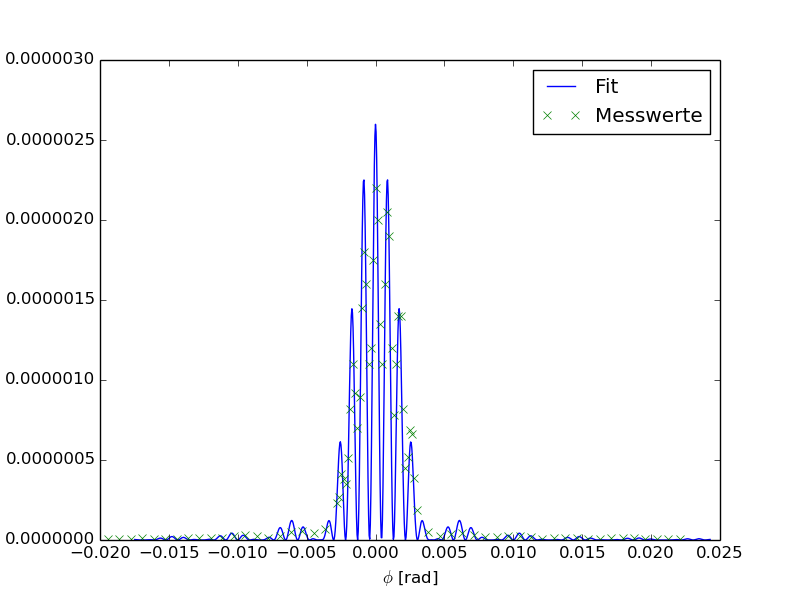
\includegraphics[scale=0.8]{plot2.png}
\caption{Beugungsmuster des Doppelspalts ($b \approx \SI{}{\milli\meter}$ und $g\approx \SI{}{\milli\meter} $)}
\label{plot0}
\end{figure} 
An diese Messwerte soll die Theoriefunktion
\begin{equation}
I(\varphi) = 4 \cdot A_0^2\cdot b^2\cos^2\left(\frac{\pi\cdot g \cdot \sin \varphi}{\lambda}\right)\cdot \operatorname{sinc}^2\left( \frac{b\cdot\sin{\varphi}}{\lambda}\right) 
\end{equation}
angepasst. Analog zum Vorgehen beim Einzelspalt werde als Startwerte für die Regressionsparameter $g$ und $b$ die mikroskopisch bestimmten Messergebnisse verwendet. Für den Amplitudenfaktor gilt:
\[
A_0 = \sqrt{\frac{I_{Max}}{4\cdot b^2}}\rm.
\]
Die Ergebnisse der Regression befinden sich in Tabelle 5. Um einen Vergleich zwischen Beugung am Einzel und am Doppelspalt zu ermöglichen zeigt Abbildung \ref{plot3} beide Beugungsmuster. Die Amplituden sind dabei jeweils auf das 0. Maximum normalisiert. 
\begin{figure}[htp]
\centering
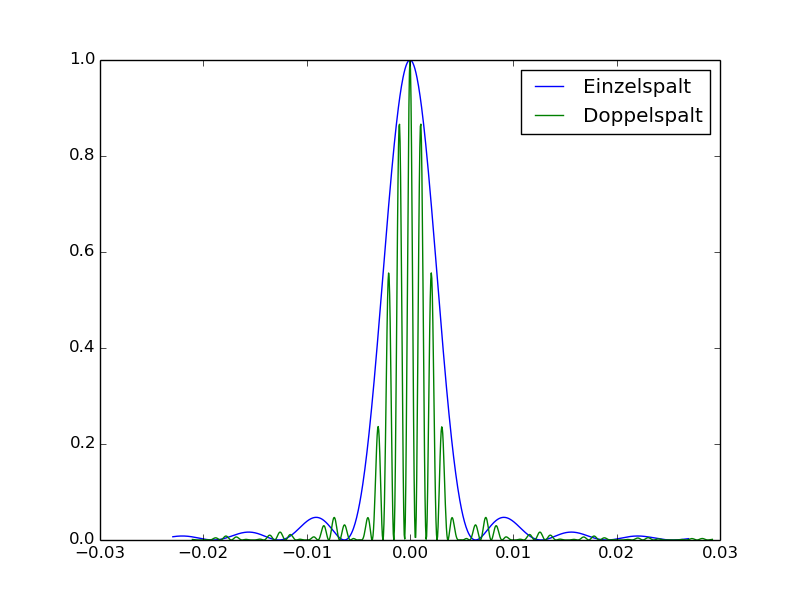
\includegraphics[scale=0.8]{/home/martin/Dokumente/SS14/Praktikum/V406/plot4.png}
\caption{Vergleich zwischen Beugung am Doppelspalt und Beugung am Einzelspalt mit näherungsweise gleicher Spaltbreite $b$.}
\label{plot3}
\end{figure}

\subsection{}
\section{Diskussion}

\section{Quellen}
\begin{enumerate}[{[}1{]}]
\item Entnommen der Praktikumsanleitung \textit{} der TU Dortmund. \\
Download am 16.06.14 unter:\\
 \url{http://129.217.224.2/HOMEPAGE/PHYSIKER/BACHELOR/AP/SKRIPT/V406.pdf}
\end{enumerate}
\section{Anhang}
\begin{itemize}
\item Auszug aus dem Messheft
\end{itemize}
\end{document}
